\documentclass[crop,tikz]{standalone}% 'crop' is the default for v1.0, before it was 'preview'
% \usetikzlibrary{...}% tikz package already loaded by 'tikz' option
\usepackage{tikz}
\usepackage{amsmath, amsthm, amssymb, amsfonts, bm}
\usetikzlibrary{shapes,arrows.meta}
\usepackage{mathptmx}
\DeclareMathAlphabet{\mathcal}{OMS}{cmsy}{m}{n}
% \DeclareMathAlphabet{\boldsymbol}{OMS}{cmsy}{m}{n}

% Talon's custom commands
\newcommand{\argmin}{\arg\!\min}
\newcommand{\me}{\mathrm{e}}
\providecommand{\e}[1]{\ensuremath{\times 10^{#1}}} 
\providecommand{\mb}[1]{\mathbf{#1}}
\providecommand{\mf}[1]{\mathfrak{#1}}
\providecommand{\mc}[1]{\mathcal{#1}}
\providecommand{\ro}{\mathbf{\mathbf{r}}_o}
\providecommand{\so}{\mathbf{\hat{s}}_o}
\providecommand{\rb}{\mathbf{r}_b}
\providecommand{\rbm}[1]{r_b^{\text{m}}}
\providecommand{\rd}{\mathbf{r}_d}
\providecommand{\rdf}{\mathpzc{r}_d}
\providecommand{\mh}[1]{\mathbf{\hat{#1}}}
\providecommand{\mbb}[1]{\mathbb{#1}}
\providecommand{\bs}[1]{\boldsymbol{#1}}
\providecommand{\bv}{\bs{\nu}}
\providecommand{\bsh}[1]{\hat{\boldsymbol{#1}}}
\providecommand{\nan}{\left(\frac{\text{NA}}{n_o}\right)}
\providecommand{\lmsum}{\sum_{l=0}^\infty\sum_{m=-l}^{l}}
\providecommand{\intr}[1]{\int_{\mbb{R}^{#1}}}
\providecommand{\ints}[1]{\int_{\mbb{S}^{#1}}}
\DeclareFontFamily{OT1}{pzc}{}
\DeclareFontShape{OT1}{pzc}{m}{it}{<-> s * [1.10] pzcmi7t}{}
\DeclareMathAlphabet{\mathpzc}{OT1}{pzc}{m}{it}
\newcommand{\eqname}[1]{\tag*{#1}}
\newcommand*\widefbox[1]{\fbox{\hspace{1em}#1\hspace{1em}}}

\tikzstyle{block} = [draw, fill=white, rectangle, minimum height=4em, minimum width=7em, align=center]

\begin{document}
  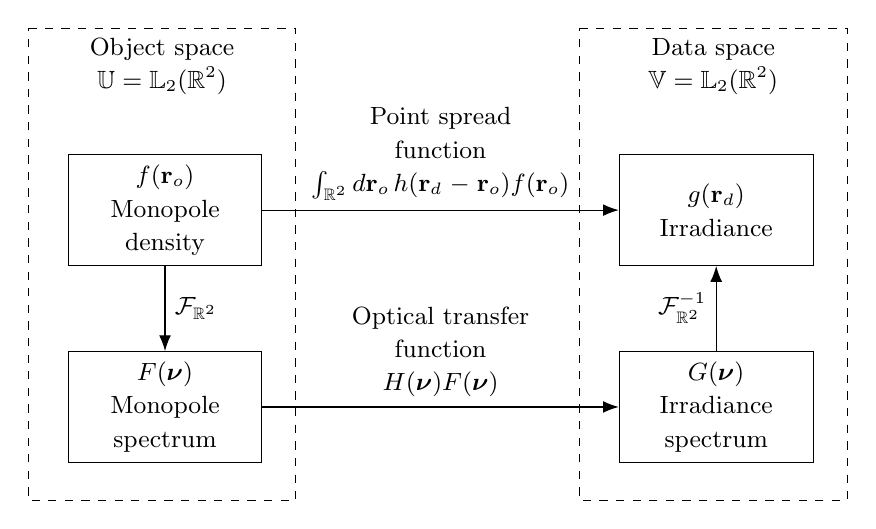
\begin{tikzpicture}[auto, node distance=2cm,>={Latex[length=2mm]}]
    \tikzset{font={\fontsize{9pt}{12}\selectfont}}
    \node [block, align=center] (den) {$f(\ro{})$\\ Monopole\\ density};
    \node [block, below of=den, node distance=2.5cm] (ds) {$F(\bs{\nu})$\\ Monopole\\ spectrum};
    \node [block,  right of=den, node distance=7cm] (irr) {$g(\rd)$\\ Irradiance};
    \node [block,  right of=ds, node distance=7cm] (is) {$G(\bs{\nu})$\\ Irradiance\\ spectrum};
    \draw [->] (den) -- node[] {$\mathcal{F}_{\mathbb{R}^2}$} (ds);
    \draw [->] (is) -- node[left] {$\mathcal{F}^{-1}_{\mathbb{R}^2}$} (irr);
    
    \draw [->] (den) -- node[text width=4cm, align=center] (cap1) {Point spread\\ function\\ $\int_{\mbb{R}^2}d\ro\, h(\rd - \ro)f(\ro)$} (irr);
    \draw [->] (ds) -- node[text width=4cm, align=center] (cap1) {Optical transfer\\ function\\ $H(\bs{\nu})F(\bs{\nu})$} (is);
    
    % Dashed box
    \draw [dashed] (den.north west) ++(-0.5cm,1.6cm) -- node[below, align=center] {Object space\\ $\mbb{U} = \mbb{L}_2(\mbb{R}^2)$} ++(3.4cm,0) -- ++(0,-6cm) -- ++(-3.4cm,0) -- ++(0, 6cm);
    \draw [dashed] (irr.north west) ++(-0.5cm,1.6cm) -- node[below, align=center] {Data space\\ $\mbb{V} = \mbb{L}_2(\mbb{R}^2)$} ++(3.4cm,0) -- ++(0,-6cm) -- ++(-3.4cm,0) -- ++(0, 6cm);
      \end{tikzpicture}
\end{document}